\chapter{TABELE ȘI FIGURI}

\section{Tabele}

Se vor evita tabelele mari; nu este permis să depășească formatul paginii.

Tabelele din lucrare trebuie să aibă o prezentare unitară. Fiecare tabel trebuie să fie numerotat și să aibă o legendă (titlu / descriere sumară). Legenda tabelului se va scrie \textbf{bold}, drept, centrat, deasupra tabelului \textbf{--} ex.: \textbf{Tabelul 3.1.} Rezultate obținute (validare).

Între un paragraf și legenda unui tabel se lasă un rând liber (12 pt); la fel între tabel și paragraful următor. Între legendă și tabel se lasă un rând liber (12 pt).

Dacă tabelul este mai mare, se poate folosi în interior scrierea la un rând, eventual și cu font mai mic de 12. Prima linie a tabelului (și/sau prima coloană, după caz) se va scrie \textbf{bold}.

În tabele se vor folosi aceleași fonturi și reguli de editare ca pentru ecuații.

Trimiterile din text la tabele se vor face scriind drept cuvântul „Tabelul” urmat de numărul acestuia.

Dacă există tabele care cuprind note, acestea se vor scrie imediat după tabel, nu la piciorul paginii și nici în corpul tabelului.

Dacă un tabel ar fi prea lung astfel încât ar depăși o pagină întreagă, atunci se va despărți, într-un mod corespunzător, în două (sau mai multe) tabele distincte.

Tabelele vor fi numerotate în continuare, pe capitole – ex.: 2.1, 2.2, ..., 3.1, 3.2, ...

Toate tabelele se vor numerota și trebuie referite în text \textbf{înainte} de prezentarea acestora. \\

În finalul acestui subcapitol este ilustrat un exemplu de tabel, acesta fiind Tabelul \ref{comp}, unde UA și WA reprezintă acuratețea neponderată, respectiv ponderată.

\vfill

\begin{table}
\centering
\caption{Rezultate obținute (validare).}
\label{comp}
\begin{tabular}{|l|r|r|}
\hline
\textbf{Model}                    & \textbf{UA [\%]} & \textbf{WA [\%]}  \\\hline
DNN (3 straturi
  ascunse, ReLU)  & 66.5             & 70.2              \\\hline
DNN (3 straturi
  ascunse, tanh)  & 66.8             & 71.0              \\\hline
CNN (5 straturi
  convoluționale) & 75.4             & 79.3              \\\hline
CNN (8 straturi
  convoluționale) & 54.2             & 58.1              \\\hline
ResNet50                          & 70.6             & 73.9              \\\hline
ResNet50V2                        & 72.3             & 75.7             \\\hline
\end{tabular}
\end{table}

\section{Figuri}

Figurile vor fi incluse în text și pot fi alb-negru sau color, cu un contrast foarte bun între nuanțele de gri sau culori, fără să depășească formatul paginii.

Fiecare figură trebuie numerotată și să aibă o legendă (titlu / descriere sumară). Legenda figurii se va scrie \textbf{bold}, drept, centrat, sub figură – ex.: \textbf{Figura 3.1.} Exemplu de evoluție a funcției cost pentru antrenare și pentru validare. Este marcat punctul în care modelul începe să manifeste supraantrenare.

Între un paragraf și o figura se lasă un rând liber (12 pt); la fel între legenda figurii și paragraful următor. Între figură și legendă se lasă un rând liber (12 pt).

În figuri se vor folosi aceleași fonturi și reguli de editare ca pentru formule.

Trimiterile din text la o anumită figură sau la mai multe figuri se vor face scriind drept cuvântul „Figura”/„Figurile” urmat de numerele acestora – ex.: Figura 3.1, Figurile 4.1-4.2.

Figurile se vor poziționa centrat, pe cât posibil în partea de sus sau de jos a paginii, dar \textbf{după} locul în care sunt referite prima oară în text.
	
 În cazul diagramelor care reprezintă variații calitative, pe axele de coordonate (la capete și în afara desenului) se vor indica doar simbolurile mărimilor în cauză; în schimb, în cazul diagramelor cantitative, axele de coordonate vor cuprinde valorile și unitățile de măsură corespunzătoare mărimilor ce variază.
	
 \textbf{Se recomandă insistent} să nu rămână spații goale mari pe pagină, înainte de o figură care s-ar poziționa la începutul paginii următoare.
	
 Figurile vor fi numerotate în continuare, pe capitole – ex.: 2.1, 2.2, ..., 3.1, 3.2, ...
	
 Toate figurile se vor numerota și trebuie referite în text \textbf{înainte} de prezentarea acestora.\\

	
În finalul acestui subcapitol este ilustrat un exemplu de figură, aceasta fiind Figura \ref{fig:exemplu}.


\begin{figure}[h]
\centering
    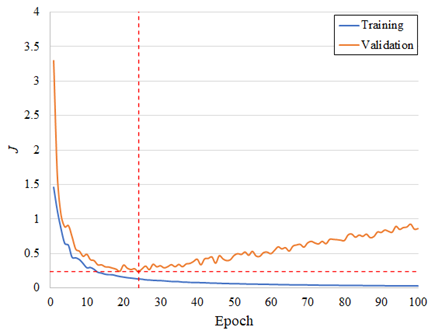
\includegraphics[width=0.7\textwidth]{figuri/Figura1.png}
    \caption{Exemplu de evoluție a funcției cost pentru antrenare și pentru validare. Este marcat punctul în care modelul începe să manifeste supraantrenare.}
    \label{fig:exemplu}
\end{figure}
